\chapter{Αποτελέσματα Προσομοιώσεων} \label{Chapter3}

\section{Επιβεβαίωση Θεωρητικών Αποτελεσμάτων} \label{Chapter3Section1}

Στην ενότητα αυτή παρουσιάζεται το σύστημα που υλοποιήθηκε στα διάφορα σενάρια προσομοιώσεων που αϰολουϑούν, τα οποία πραγματοποιήϑηϰαν σε περιβάλλον MATLAB. Για την απόδειξη των θεωρητικών αποτελεσμάτων, χρησιμοποιήθηκε το αναλυτικό μοντέλο προσομοίωσης \textbf{KUKA LWR4+}, πανομοιότυπο και για τους δύο ρομποτικούς βραχίονες του Ηγέτη και του Ακόλουθου για τις 4 πρώτες αρθρώσεις τους. Και οι δύο λειτουργούν με περίοδο δειγματοληψίας στον κύκλο ελέγχου στα \textbf{[1ms]}. Επιπλέον, θεωρούμε στα πλάισια της προσομοιώσεις το διάνυσμα των βαρυτικών ροπών $\mathbf{G}_{\kappa} = 0^{m}$. Στο Πίνακα~\bref{table:concise_table} καταγράφονται οι τιμές που θέσαμε στις διάφορες μεταβλητές του σχεδιαστικού ελέγχου μετά από πολλαπλές δοκιμές για να σκιαγραφήσουμε το κάτα πόσο οι δύο προκλήσεις που τεκμηριώσαμε στην Ενότητα~\bref{Chapter1Section3}, αντιμετωπίζονται αποτελεσματικά. Στο Ηγέτη έχει δωθεί χαμηλή απτική ανάδραση, μεγάλα όρια γωνιών αρθρώσεων και ταχυτήτων, καθώς και μεγάλες ροπές εισόδου, για να καταφανούν τα επιδιωκωμένα αποτελέσματα από πλευράς του Ακόλουθου.
Οι ασκούμενες δυνάμεις από τον άνθρωπο-χειριστή θα είναι:
\begin{align*}
    \mathbf{\tau}_{h} = \big[-4sin(0.75t),\quad 4sin(0.75t), \quad &4sin(0.75t), \quad -4sin(0.75t), \\ &\qquad0.1sin(0.75t), \quad0.1cos(0.75t), 0\big]
\end{align*}

\bigskip
Για την σχεδιαστική παράμετρο $Q_{F_{2}}$ θεωρείται πως μετά από πολλές δοκιμές βρίσκονται τέτοιες που ικανοποιούν την συνθήκη \bref{QF2}. Οι τιμές των υπολοίπων παραμέτρων του σχήματος ελέγχου επιλέγονται ώστε να εξασφαλίζονται ταυτόχρονα η ποιοτιϰή εξέλιξη των σφαλμάτων εξόδου εντός των αντίστοιχων φαϰέλων επίδοσης, η παραγωγή αποδεϰτών τιμών εισόδου ελέγχου ϰαι η όσο το δυνατόν μεγαλύτερη ολική ευστάθεια του συστήματος κλειστού βρόχου.

\begin{table}[H]
    \centering
    \caption{Γωνίες, Κέρδη, και Σχεδιαστικές Παράμετροι για τον Ηγέτη και τον Ακόλουθο}
    \begin{tabular}{|c|c|c|c|c|}
    \hline
    \textbf{Παράμετρος} & \textbf{Άρθρωση 1} & \textbf{Άρθρωση 2} & \textbf{Άρθρωση 3} & \textbf{Άρθρωση 4} \\ \hline
    \textbf{Αρχικές Γωνίες Ηγέτη [rad]} & -0.47 & 0.97 & -0.28 & -1.1 \\ \hline
    \textbf{Αρχικές Γωνίες Ακόλουθου [rad]} & -0.09 & 1.5 & 0.2 & -1.5 \\ \hline
    \textbf{Αρχικές Ταχύτητες Ακόλουθου [rad/s]} & 0 & 0 & 0 & 0 \\ \hline
    \textbf{Αρχικές Ταχύτητες Ακόλουθου [rad/s]} & 0 & 0 & 0 & 0 \\ \hline
    \textbf{Περιορισμοί $\rho^{0}_{F_{1}}$(\bref{rhoF10>})} & >0.38 & >0.53 & >0.48 & >0.4 \\ \hline
    \textbf{Σχεδιαστικές Παράμετροι $\rho^{0}_{F_{1,i}}$(\bref{rhoF10>})} & 1.0 & 1.0 & 1.0 & 1.0 \\ \hline
    \textbf{Σχεδιαστικές Παράμετροι $\rho^{\infty}_{F_{1,i}}$(\bref{rhoinfty})} & 0.02 & 0.02 & 0.02 & 0.02 \\ \hline
    \textbf{Σχεδιαστικές Παράμετροι $\lambda$(\bref{lambda})} & 0.02 & 0.02 & 0.02 & 0.02 \\ \hline
    \textbf{Κέρδη $k_{\zeta_{1}}$(\bref{kzeta1})} & 1.3 & 1.3 & 1.3 & 1.3 \\ \hline
    \textbf{Κέρδη $k_{L_{1}}$(\bref{kappa1})} & 7.0 & 7.0 & 7.0 & 7.0 \\ \hline
    \textbf{Κέρδη $k_{F_{1}}$(\bref{kappa1})} & 1.0 & 1.0 & 1.0 & 1.0 \\ \hline
    \textbf{Κέρδη $k_{O_{1}}$(\bref{kappa1})} & 1.0 & 1.0 & 1.0 & 1.0 \\ \hline
    \textbf{Σχεδιαστικές Παράμετροι $\gamma_{L_{1}}$(\bref{gamma1})} & 0.4 & 0.4 & 0.4 & 0.4 \\ \hline
    \textbf{Σχεδιαστικές Παράμετροι $\rho_{F_{2}}$} & 1.8 & 2.2 & 2.0 & 1.8 \\ \hline
    \textbf{Κέρδη $k_{\zeta_{2}}$(\bref{kzeta2})} & 1.3 & 1.3 & 1.3 & 1.3 \\ \hline
    \textbf{Κέρδη $k_{L_{2}}$(\bref{kappa2})} & 5.0 & 7.0 & 7.0 & 5.0 \\ \hline
    \textbf{Κέρδη $k_{F_{2}}$(\bref{kappa2})} & 7.0 & 7.0 & 7.0 & 7.0 \\ \hline
    \textbf{Κέρδη $k_{O_{2}}$(\bref{kappa2})} & 1 & 1 & 1 & 1 \\ \hline
    \textbf{Κέρδη $k_{H}$(\bref{uH})} & 1.0 & 1.0 & 1.0 & 1.0\\ \hline
    \textbf{Σχεδιαστικές Παράμετροι $\gamma_{L_{2}}$(\bref{gamma2})} & 0.3 & 0.3 & 0.3 & 0.3 \\ \hline
    \textbf{Διαχωριστική γραμμή $Q_{S}$((\bref{QsQF1}))} & 1.1 & 1.6 & 0.4 & 1.8\\ \hline
    \textbf{Περιορισμός Εξόδου $Q_{F_1}$(\bref{QsQF1})} & 1.5 & 2.0 & 0.8 & 2.1\\ \hline
    \textbf{Σχεδιαστικές Παράμετροι $Q_{F_2}$(\bref{QF2})} & 2.0 & 2.0 & 2.0 & 2.0\\ \hline
    \end{tabular}
    \label{table:concise_table}
    \end{table}

\bigskip
Σε κάθε σενάριο, οι αρθρώσεις του Ηγέτη υπερβαίνουν τους προκαθορισμένους περιορισμούς στην έξοδο του Ακόλουθου. Αυτό γίνεται με στόχο να επιβεβαιωθεί η επιτυχής αλλαγή προτεραιότητας από την ακριβή αναπαράσταση της τροχιάς του Ηγέτη στην ασφάλεια και ακεραιότητα του ρομποτικού βραχίονα του Ακόλουθου, και αντίστροφα. Αυτή η προσέγγιση αποτελεί την κύρια στρατηγική σχεδιασμού και τον ελεγκτικό στόχο της παρούσας εργασίας.

\bigskip
Παρατίθεται το παρακάτω σενάριο με καθυστέρηση που ικανοποιεί την Υπόθεση~\bref{hyp:3}
\begin{gather*}
    T_{D}(t) = 0.5 + 0.5\sin(t)\ \text{sec}
\end{gather*}
η οποία έχει άνω φράγμα $\bar{T}_{D} = 1\ \text{s}$ και είναι συνεχής παντού.

\begin{figure}[H]
    \centering
    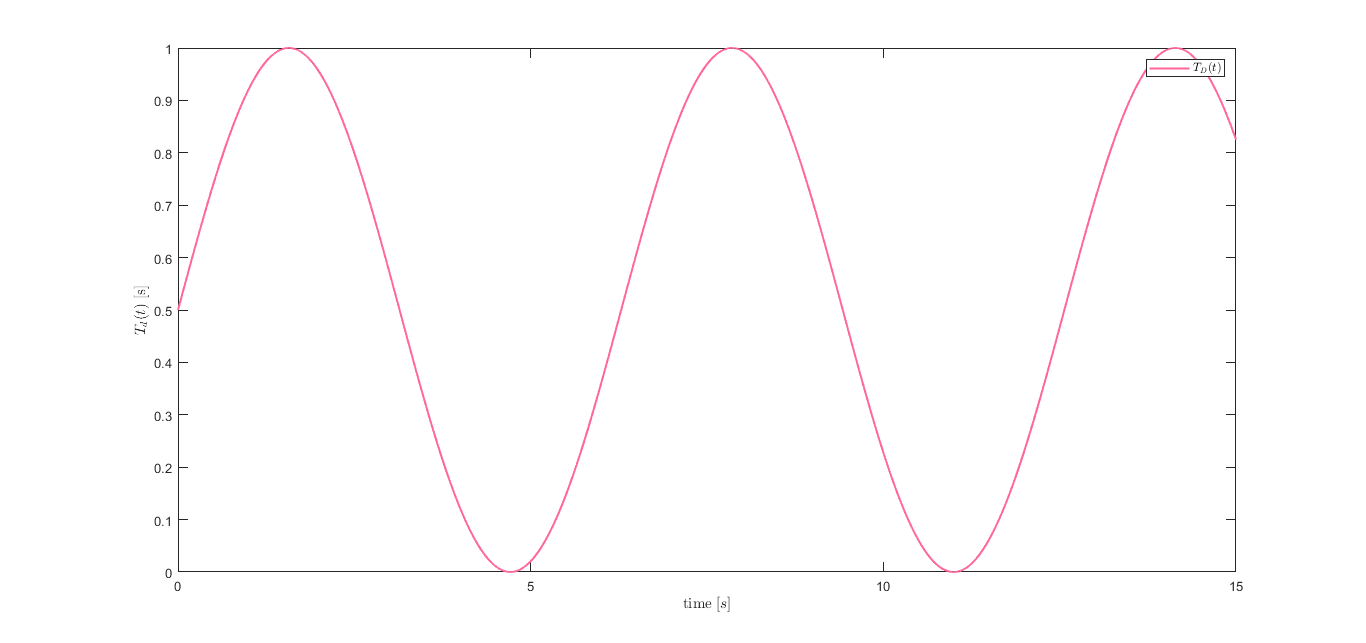
\includegraphics[width=1\linewidth]{Chapters/Chapter3/Figures/Sim1Fig1.png}
    \caption[Σενάριο Καθυστέρησης που ικανοποιεί τις Υποθέσεις]{Σενάριο Καθυστέρησης που ικανοποιεί τις Υποθέσεις}
    \label{Sim1Fig1}
\end{figure}

\begin{figure}[H]
    \centering
    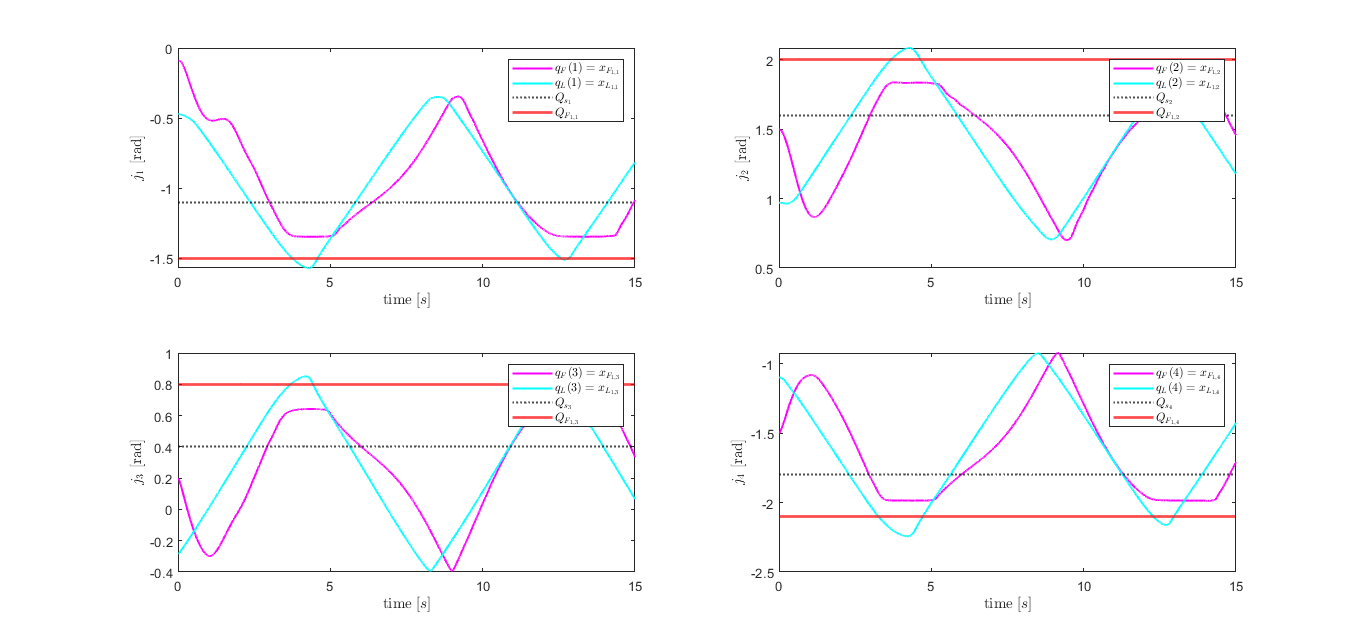
\includegraphics[width=1\linewidth]{Chapters/Chapter3/Figures/Sim1Fig2.png}
    \caption{Οι γωνίες των αρθρώσεων του \textit{Ακόλουθου} $x_{F_{1,i}}(t)$ μαζί με τις γωνίες των αρθρώσεων του \textit{Ηγέτη} $x_{L_{1,i}}(t)$.}
    \label{Sim1Fig2}
\end{figure}

\begin{figure}[H]
    \centering
    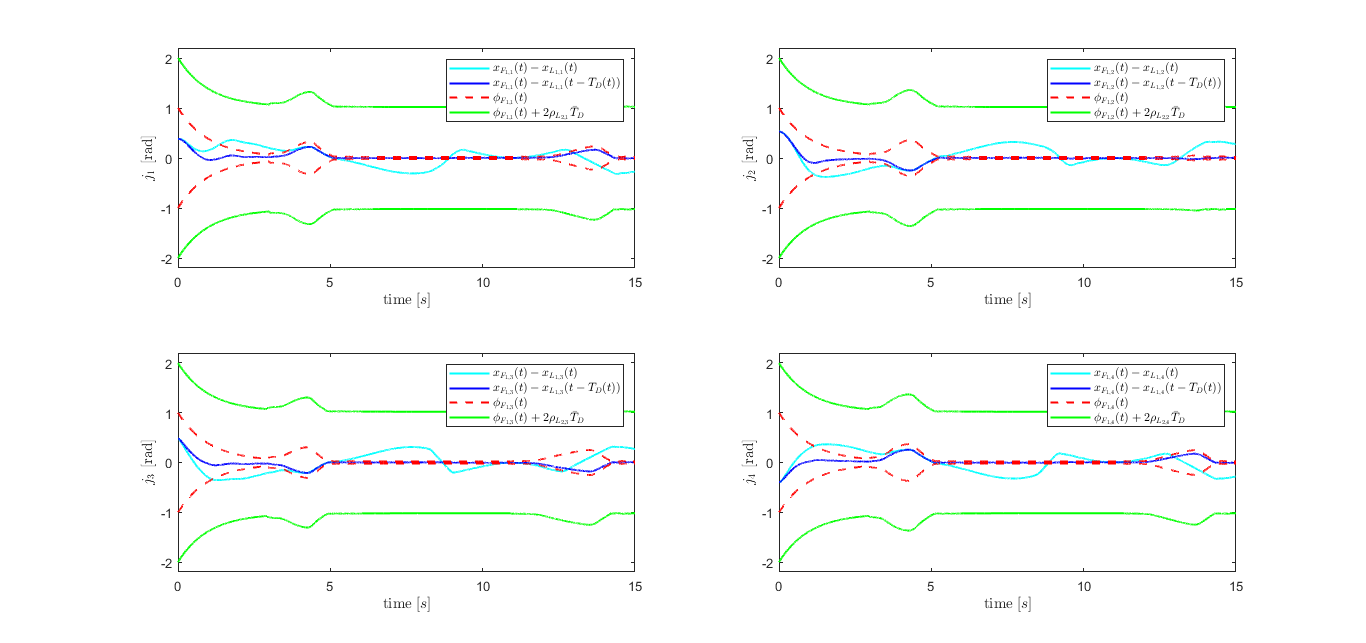
\includegraphics[width=1\linewidth]{Chapters/Chapter3/Figures/Sim1Fig3.png}
    \caption{Τα σφάλματα παρακολούθησης $x_{F_{1,i}}(t) - x_{L_{1,i}}(t - T_{D})$ και $x_{F_{1,i}}(t) - x_{L_{1,i}}(t)$ μαζί με τις αντίστοιχες συναρτήσεις επίδοσης $\phi_{F_{1,i}}(t)$.}
    \label{Sim1Fig3}
\end{figure}
\begin{figure}[!ht]
    \centering
    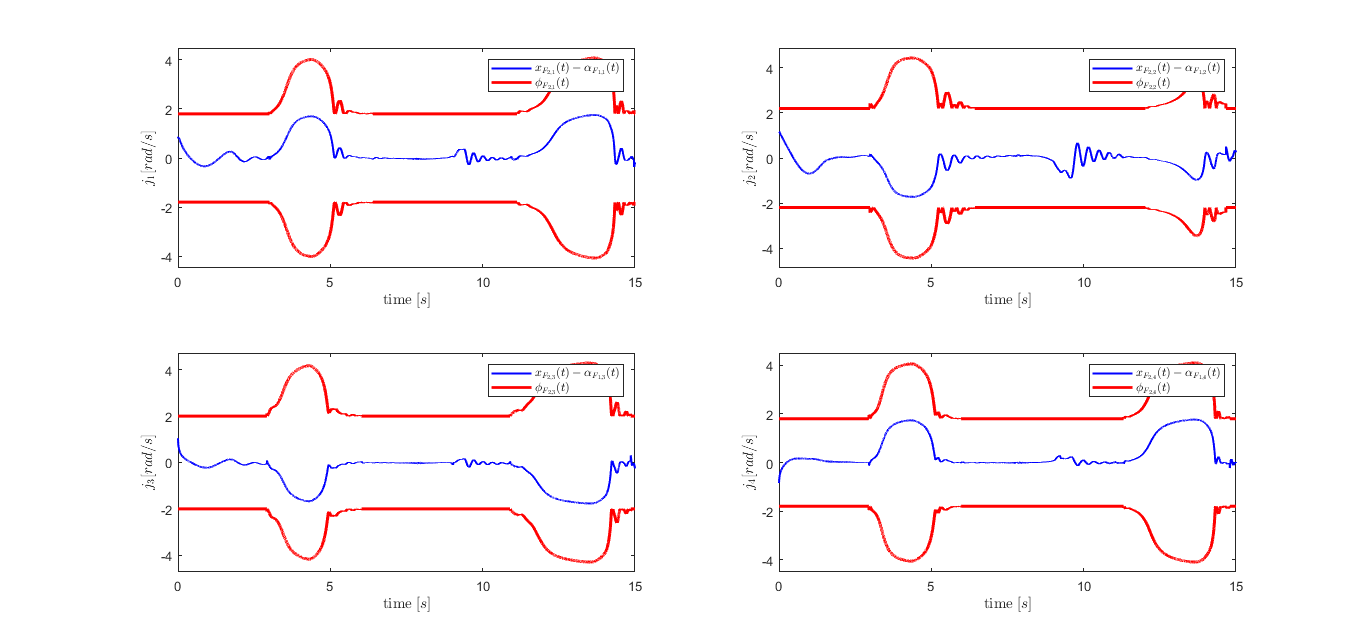
\includegraphics[width=1\linewidth]{Chapters/Chapter3/Figures/Sim1Fig4.png}
    \caption{Τα ενδιάμεσα σφάλματα $x_{F_{2,i}}(t) - \alpha_{F_{1,i}}(t)$ μαζί με τα αντίστοιχα όρια επίδοσης $\phi_{F_{2,i}}(t)$.}
    \label{Sim1Fig4}
\end{figure}

\begin{figure}[H]
    \centering
    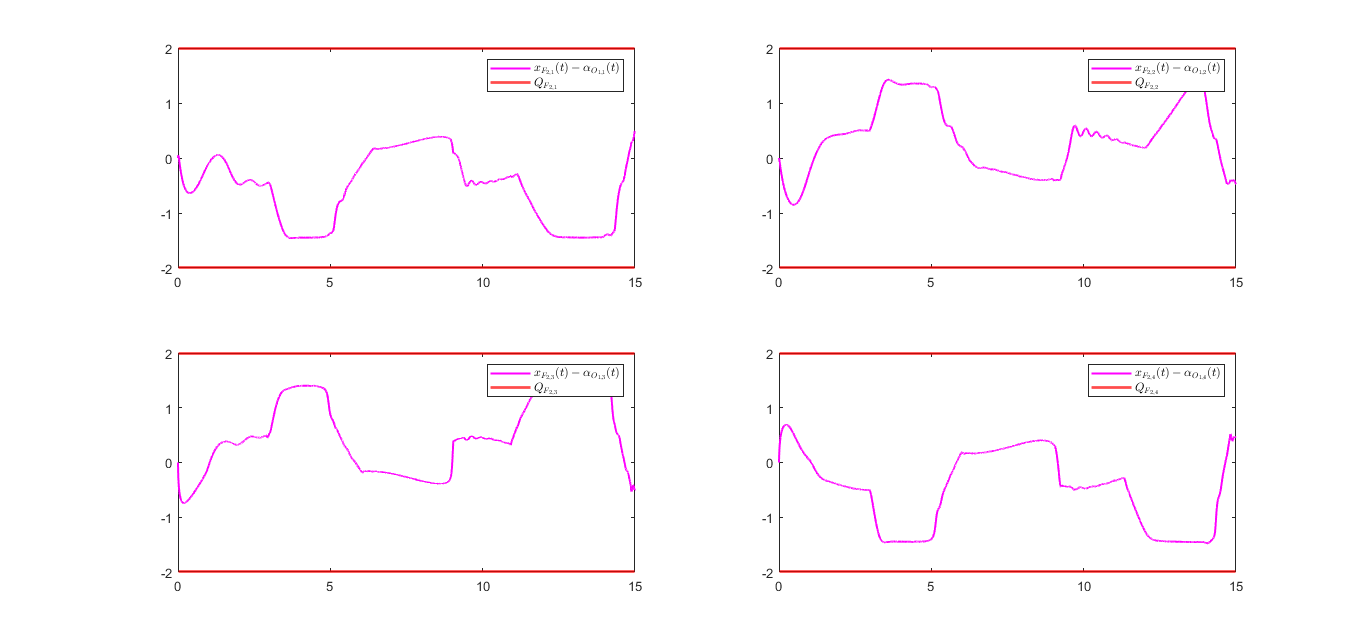
\includegraphics[width=1\linewidth]{Chapters/Chapter3/Figures/Sim1Fig5.png}
    \caption{Τα ενδιάμεσα σφάλματα $x_{F_{2,i}}(t) - \alpha_{O_{1,i}}(t)$ μαζί με τα αντίστοιχα όρια επίδοσης $Q_{F_{2,i}}$.}
    \label{Sim1Fig5}
\end{figure}



\begin{figure}[H]
    \centering
    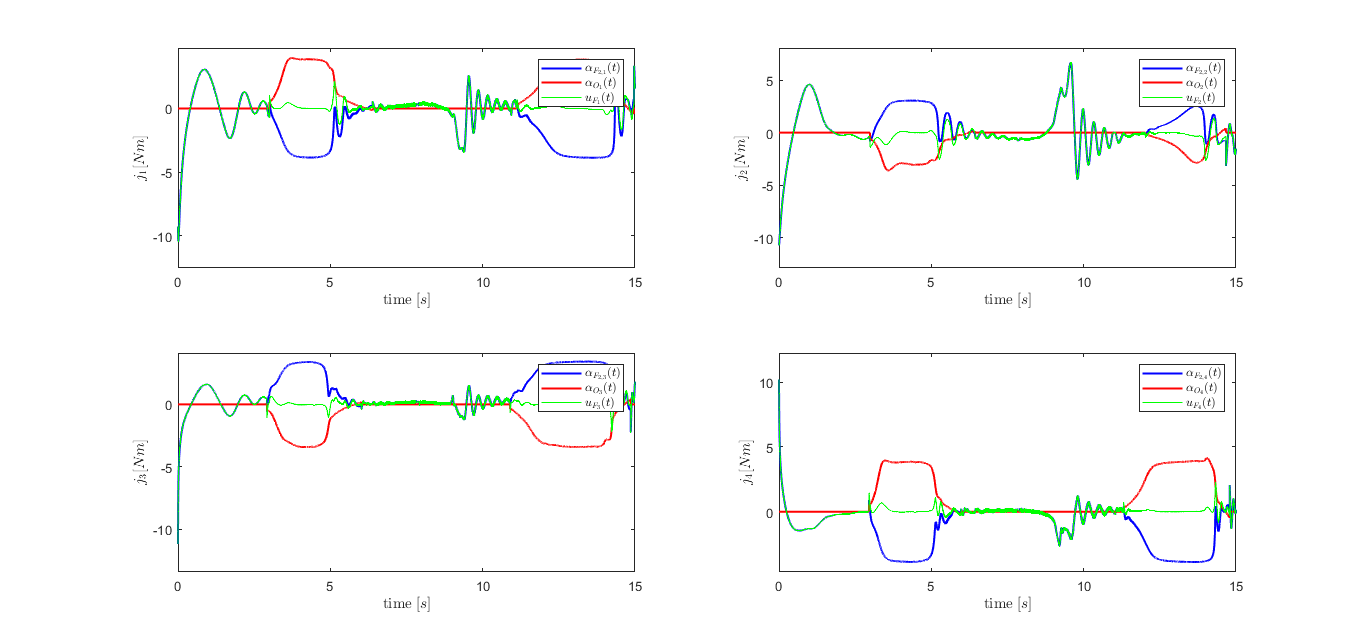
\includegraphics[width=1\linewidth]{Chapters/Chapter3/Figures/Sim1Fig6.png}
    \caption{Η είσοδος ελέγχου του Ακόλουθου $u_{F_{i}}(t)$.}
    \label{Sim1Fig6}
\end{figure}

\begin{figure}[H]
    \centering
    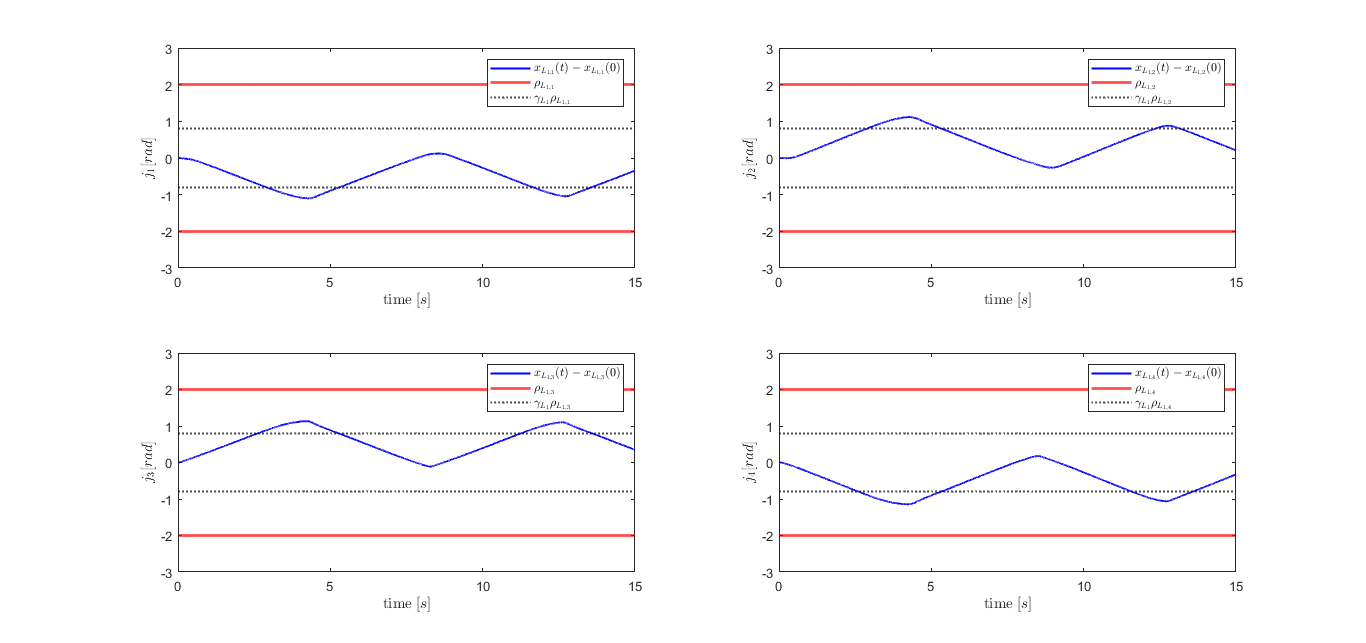
\includegraphics[width=1\linewidth]{Chapters/Chapter3/Figures/Sim1Fig7.png}
    \caption{Τα σφάλματα $x_{L_{1,i}}(t) - x_{L_{1,i}}(0)$ μαζί με τα αντίστοιχα όρια επίδοσης $\rho_{L_{1,i}}$.}
    \label{Sim1Fig7}
\end{figure}



\begin{figure}[H]
    \centering
    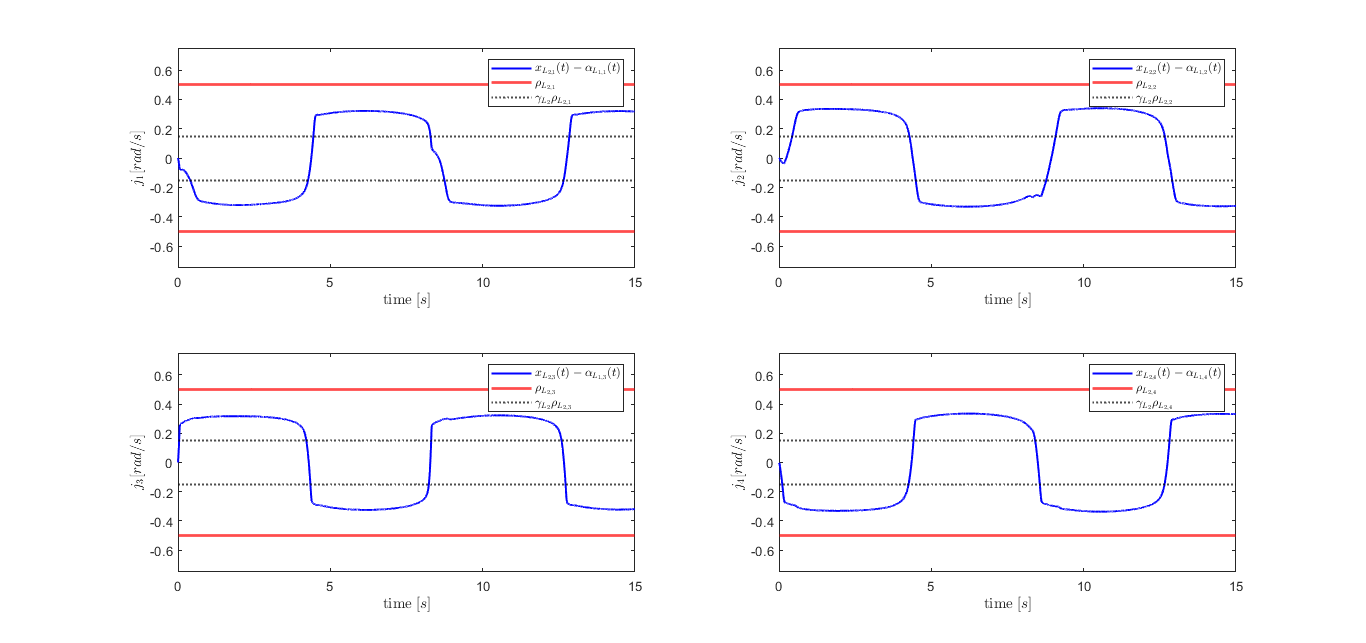
\includegraphics[width=1\linewidth]{Chapters/Chapter3/Figures/Sim1Fig8.png}
    \caption{Τα σφάλματα $x_{L_{2,i}}(t) - \alpha_{L_{1,i}}(t)$ μαζί με τα αντίστοιχα όρια επίδοσης $\rho_{L_{2,i}}$.}
    \label{Sim1Fig8}
\end{figure}

\begin{figure}[H]
    \centering
    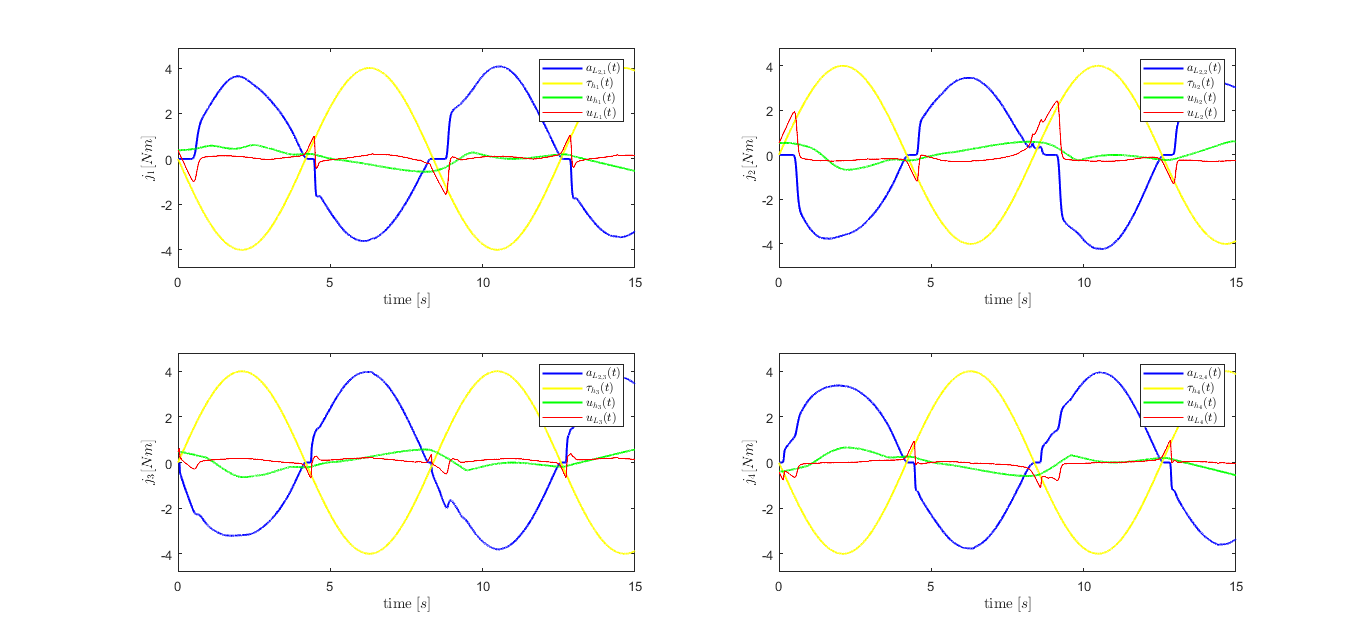
\includegraphics[width=1\linewidth]{Chapters/Chapter3/Figures/Sim1Fig9.png}
    \caption{Η είσοδος ελέγχου στον \textit{Ηγέτη} $u_{L_{i}}(t) = \alpha_{L_{2,i}}(t) + u_{H_{i}}(t)$ μαζί με τις δυνάμεις που ασκεί ο άνθρωπος πάνω του $\tau_{h_{i}}$.}
    \label{Sim1Fig9}
\end{figure}

\begin{observation}\label{fig:obs:1}
Στο σχήμα (\bref{Sim1Fig2}) βλέπουμε πως η ακριβής αναπαράσταση της καθυστερημένης τροχιάς του Ηγέτη στην \textbf{ΠΑΑ} με την παράλληλη αποφυγή του περιορισμού εξόδου στην \textbf{ΠΚΑ} με τρόπο αντίστοιχο με αυτό που απεικονίζεται στο Σχήμα~\bref{control_concept}, καταδεικνύει την επιτυχία του σχεδιαστικού ελέγχου στην αναδοχή προτεραιότητας στην συμπεριφορά του Ακόλουθου, έτσι ώστε να ακολουθεί πιστά τον Ηγέτη αλλά και να παραμένει ασφαλής όταν το πρώτο είναι αδύνατο.
\end{observation}

\bigskip
\begin{observation}\label{fig:obs:2}
Στο Σχήμα~\bref{Sim1Fig6} απεικονίζεται η είσοδος ελέγχου του Ακόλουθου. Όταν ο Ακόλουθος βρίσκεται στην Περιοχή Κινδύνου Ακόλουθου (ΠΚΑ), η είσοδος ελέγχου περιορίζεται, καθώς δίνεται προτεραιότητα στην ασφάλεια του συστήματος. Με την επιστροφή του Ακόλουθου στην Περιοχή Ασφαλείας Ακόλουθου (ΠΑΑ), και μετά από σύντομα μεταβατικά φαινόμενα, η είσοδος ελέγχου επανέρχεται, επιτρέποντας την αξιόπιστη αναπαράσταση της καθυστερημένης τροχιάς του Ηγέτη. Επιπλέον, στην Απόδειξη~\bref{proof_of_the:main} του Θεωρήματος~\bref{the:main} αποδείξαμε ότι η παρακολούθηση παραμένει φραγμένη καθόλη την διάρκεια του διμερούς τηλεχειρισμού, ενώ ο παράγοντας $u_{O}$ που προστέθηκε για την εξασφάλιση της ασφάλειας του Ακόλουθου, τείνει στο άπειρο όσο ο Ακόλουθος πλησιάζει τον περιορισμό $Q_{F_{1, i}}$.
\end{observation}

\bigskip
\begin{observation}\label{fig:obs:3}
Στα σχήματα (\bref{Sim1Fig3}) και (\bref{Sim1Fig4}) παρουσιάζονται τα σφάλματα παρακολούθησης γωνιών αλλά και ταχυτήτων, υπό τις τρέχουσες τροποποιημένες συναρτήσεις επίδοσης (\bref{phiF1_define}), (\bref{phiF2_define}), οι οποίες αυξάνουν τα όριά τους καθώς ο Ακόλουθος βρίσκεται εντός της \textbf{ΠΚΑ} για την διατήρηση της ευστάθειας. Αυτό έχει ως αποτέλεσμα την διατήρηση του Ελέγχου Προδιαγεγραμμένης Απόκρισης καθόλη την διάρκεια του ελέγχου.
\end{observation}

\bigskip
\begin{observation}\label{fig:obs:4}
Στα σχήματα (\bref{Sim1Fig7})-(\bref{Sim1Fig9}) παρουσιάζεται η συμπεριφορά του Ηγέτη, ανεπηρέαστη από την αλλαγή στρατηγικής από την πλευρά του Ακόλουθου εξαιτίας της χαμηλής απτικής ανάδρασης $u_{H}$(\bref{uH}). Με την αύξηση της τελευταίες, η δραστηριότητα του Ακόλουθου θα επιδρούσε στον Ηγέτη σε βαθμό που θα τον αποθάρρυνε από το να συνεχίσει την τροχιά του μακριά από την Περιοχή Ασφαλείας Ακόλουθου (ΠΑΑ).
\end{observation}

\section{Έλεγχος Ευρωστίας} \label{Chapter3Section3}
Καθώς η Υπόθεση~\bref{hyp:3} αποτελεί ικανή και όχι αναγκαία συνθήκη για την επίτευξη του στόχου ελέγχου και τίθεται κρίσιμο να εξεταστεί σε τι βαθμό καθίσταται αυτή περιοριστική, στα δύο επακόλουθα σενάρια θα μελετηθεί η ευρωστία του ελεγχόμενου συστήματος κλειστού βρόχου ως προς μεσαία και ακραία παραβίαση της υπόθεσης. Αυτό θα υλοποιηθεί με την σχεδίαση χρονική καθυστέρησης που $\dot{T}_D(t) > 1$. Από το έργο \cite{bresch2018robust}, φαίνεται εφικτή η διατήρηση της ευστάθειας, μάλλον και των στόχων ελέγχου, χωρίς καμία εγγύηση γι'αυτό.
Για την απόπειρα αυτή, καθίσταται σαφές η αύξηση του τελικού ορίου των συναρτήσεων επίδοσης $\rho^{\infty}_{F_{1,i}}$ από $\mathbf{0.02}$ σε $\mathbf{0.2}$ για όλες τις αρθρώσεις. Η πιο χαλαρή αυτή αντιμετώπιση του προβλήματος παρακολούθησης είναι ικανή να επιφέρει αποτελέσματα.

\bigskip
Στο σενάριο μέτριας παραβίασης θα χρησιμοποιηθεί η καθυστέρηση με άνω φράγμα $\bar{T}_{D} = 0.8\ \text{s}$.

\begin{figure}[H]
    \centering
    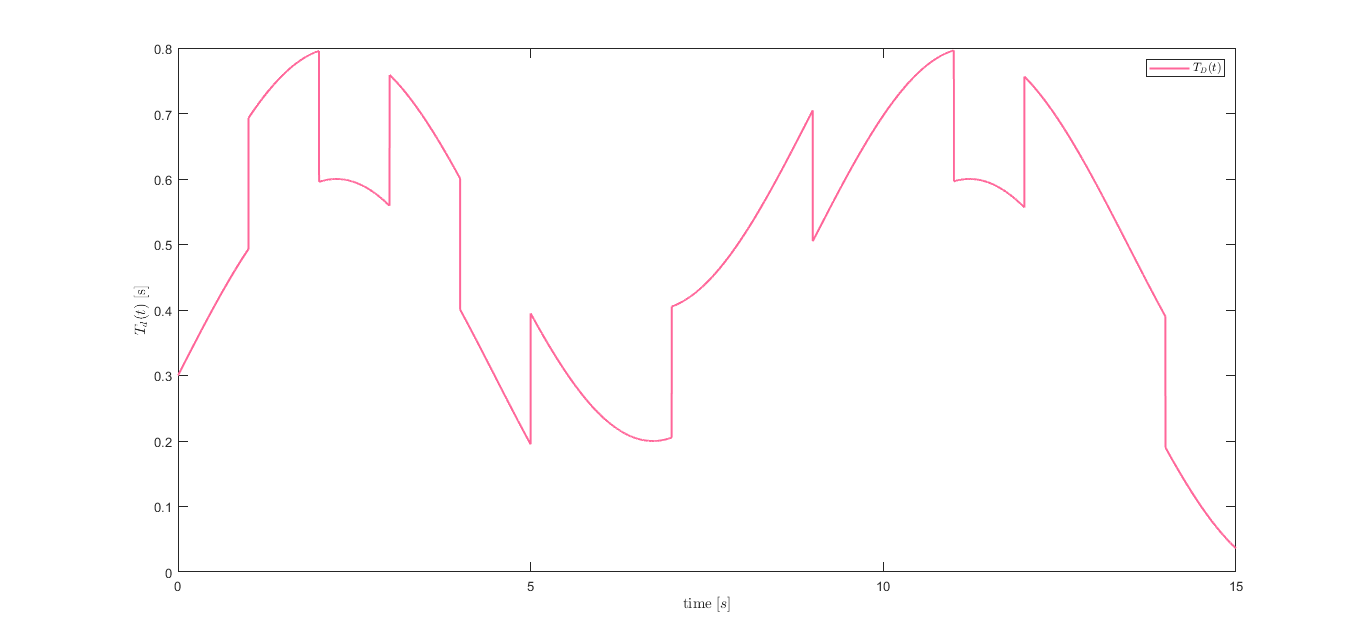
\includegraphics[width=1\linewidth]{Chapters/Chapter3/Figures/Sim2Fig1.png}
    \caption[Σενάριος μέτρια παραβίασης συνθηκών χρονικών καθυστερήσεων]{Σενάριο μέτριας παραβίασης συνθηκών χρονικών καθυστερήσεων}
    \label{Sim2Fig1}
\end{figure}

\begin{figure}[H]
    \centering
    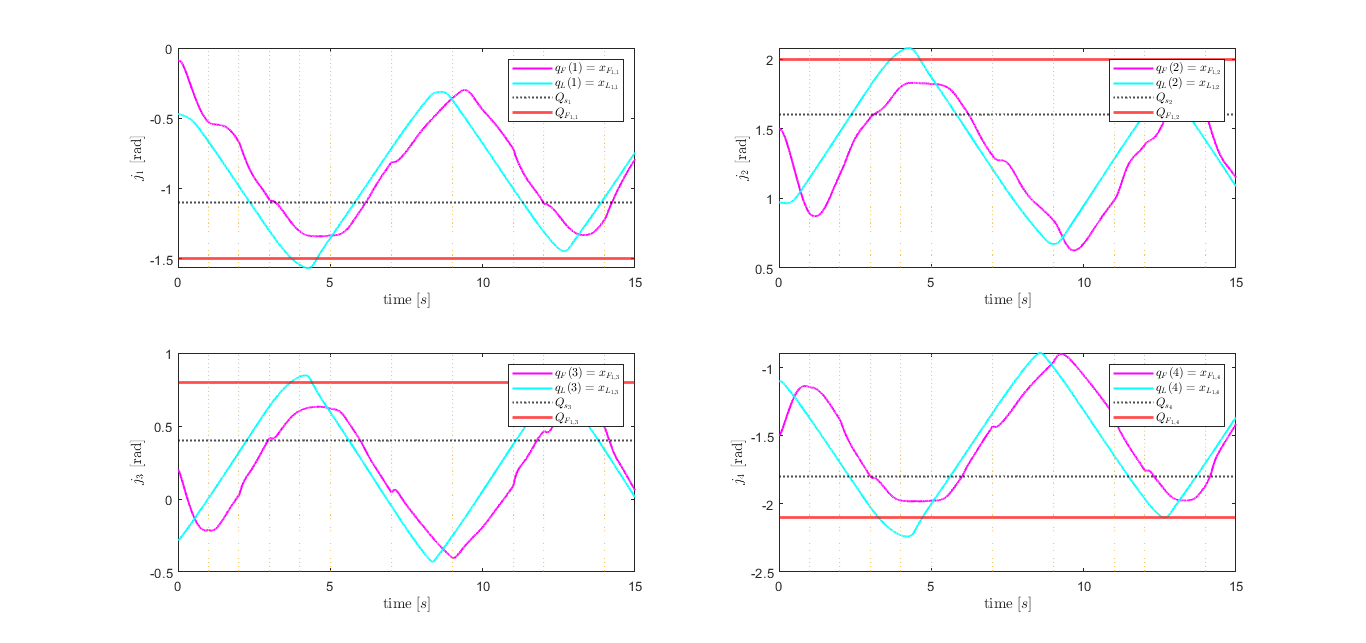
\includegraphics[width=1\linewidth]{Chapters/Chapter3/Figures/Sim2Fig2.png}
    \caption{Οι γωνίες των αρθρώσεων του \textit{Ακόλουθου} $x_{F_{1,i}}(t)$ μαζί με τις γωνίες των αρθρώσεων του \textit{Ηγέτη} $x_{L_{1,i}}(t)$.}
    \label{Sim2Fig2}
\end{figure}

\begin{figure}[H]
    \centering
    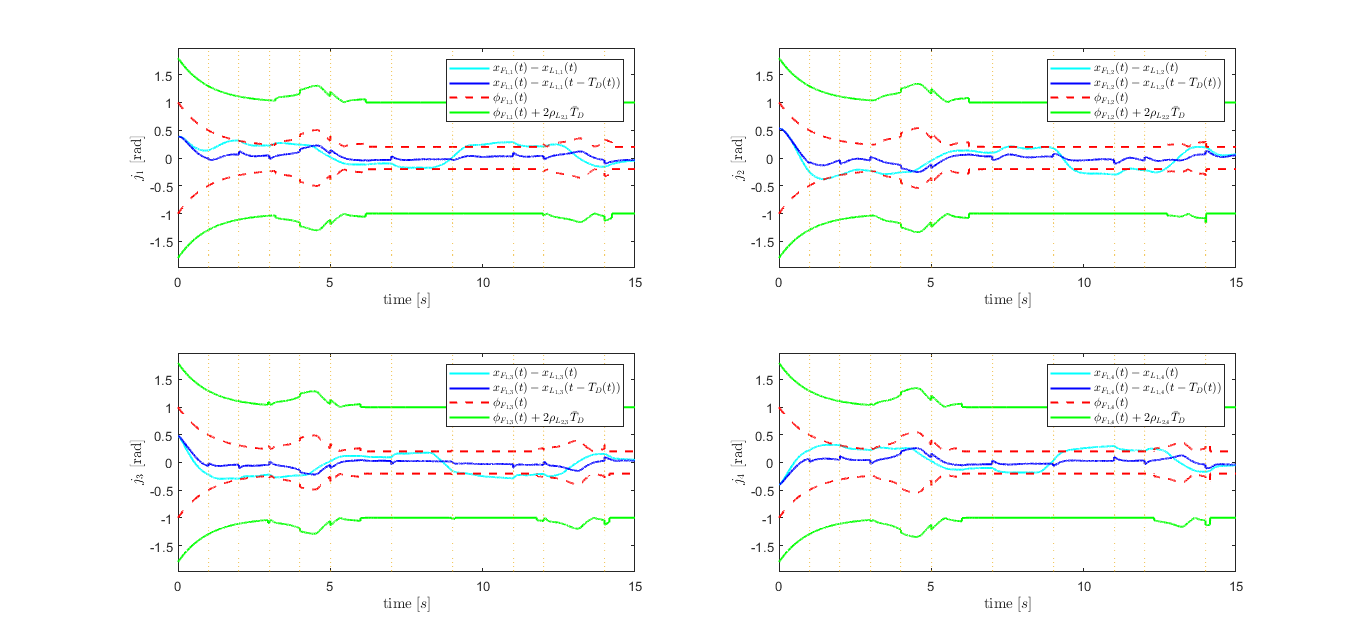
\includegraphics[width=1\linewidth]{Chapters/Chapter3/Figures/Sim2Fig3.png}
    \caption{Τα σφάλματα παρακολούθησης $x_{F_{1,i}}(t) - x_{L_{1,i}}(t - T_{D})$ και $x_{F_{1,i}}(t) - x_{L_{1,i}}(t)$ μαζί με τις αντίστοιχες συναρτήσεις επίδοσης $\phi_{F_{1,i}}(t)$.}
    \label{Sim2Fig3}
\end{figure}

\begin{figure}[H]
    \centering
    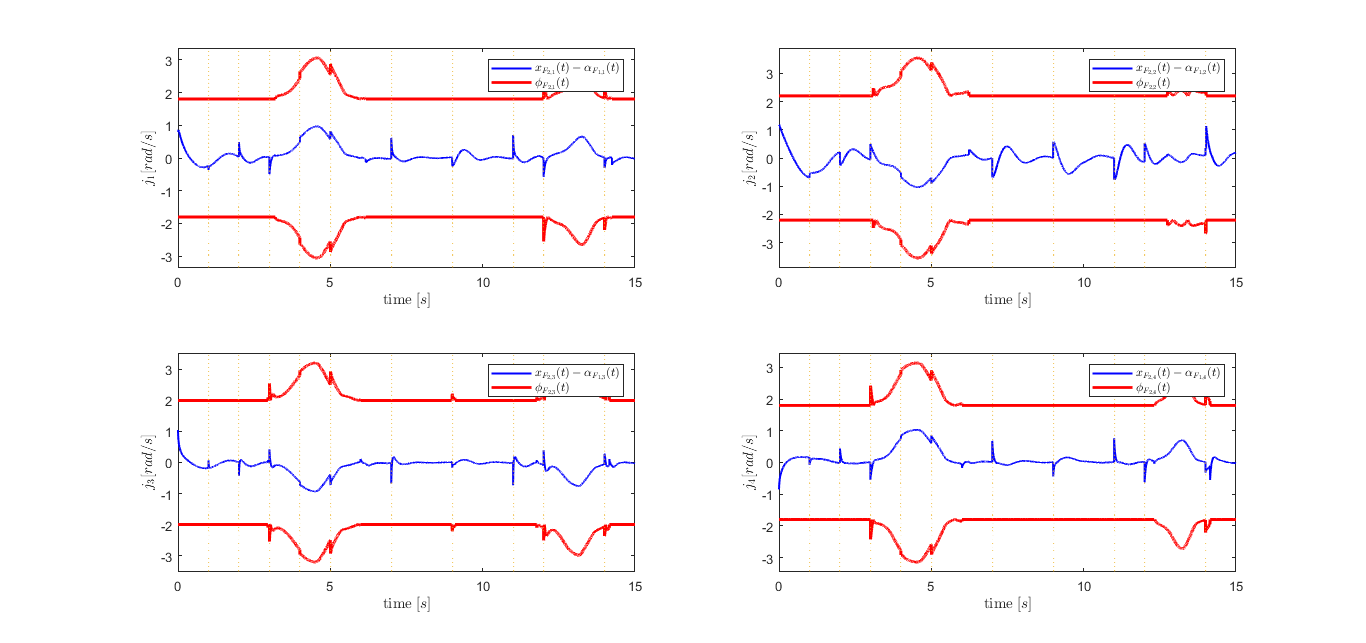
\includegraphics[width=1\linewidth]{Chapters/Chapter3/Figures/Sim2Fig4.png}
    \caption{Τα ενδιάμεσα σφάλματα $x_{F_{2,i}}(t) - \alpha_{F_{1,i}}(t)$ μαζί με τα αντίστοιχα όρια επίδοσης $\phi_{F_{2,i}}(t)$.}
    \label{Sim2Fig4}
\end{figure}

\begin{figure}[H]
    \centering
    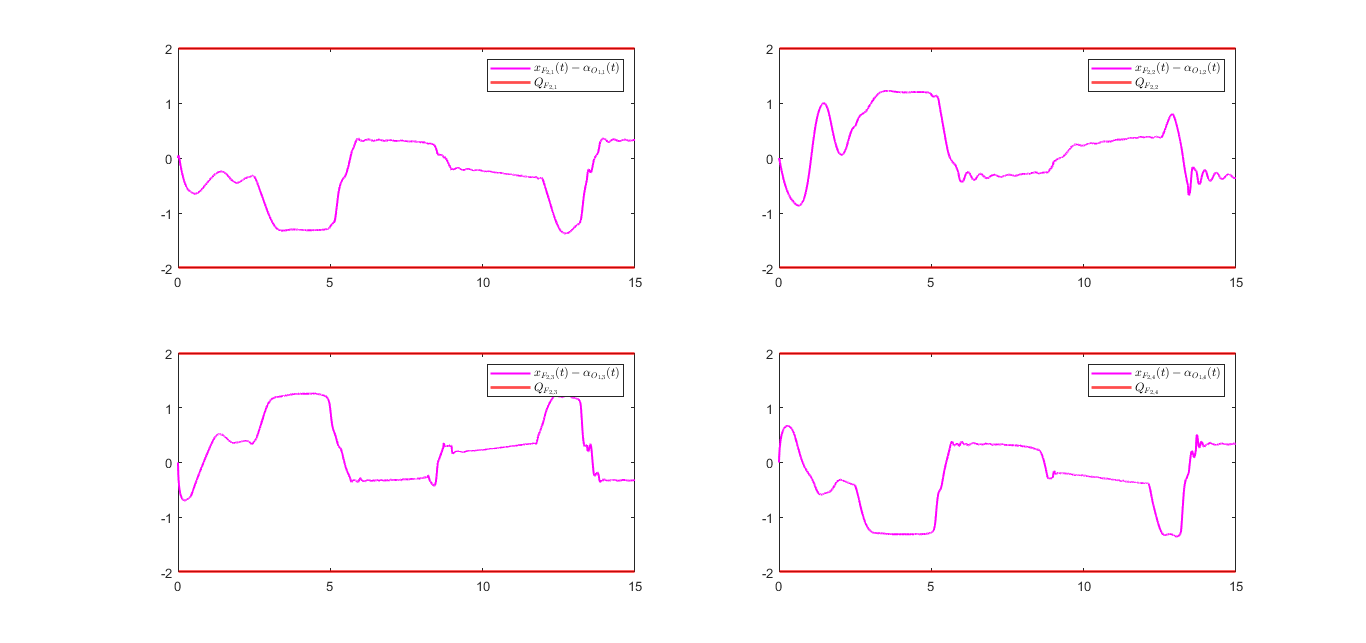
\includegraphics[width=1\linewidth]{Chapters/Chapter3/Figures/Sim2Fig5.png}
    \caption{Τα ενδιάμεσα σφάλματα $x_{F_{2,i}}(t) - \alpha_{O_{1,i}}(t)$ μαζί με τα αντίστοιχα όρια επίδοσης $Q_{F_{2,i}}$.}
    \label{Sim2Fig5}
\end{figure}



\begin{figure}[H]
    \centering
    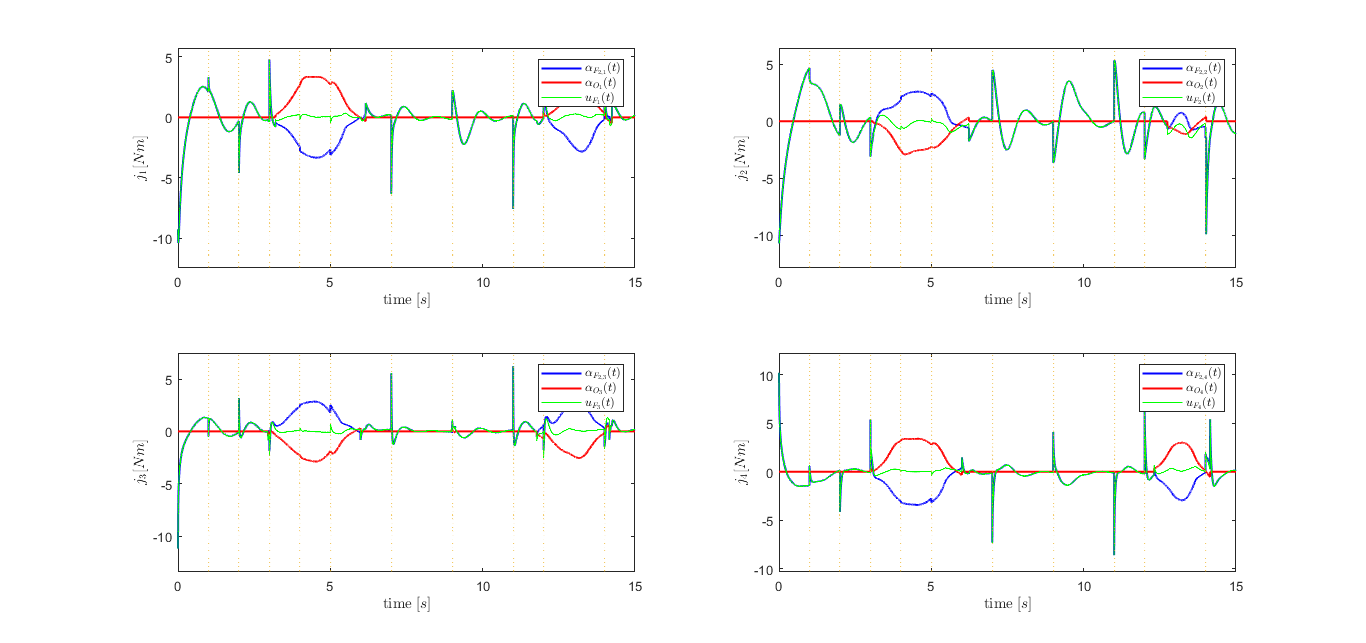
\includegraphics[width=1\linewidth]{Chapters/Chapter3/Figures/Sim2Fig6.png}
    \caption{Η είσοδος ελέγχου του \textit{Ακόλουθου} $u_{F_{i}}(t)$.}
    \label{Sim2Fig6}
\end{figure}

\begin{figure}[H]
    \centering
    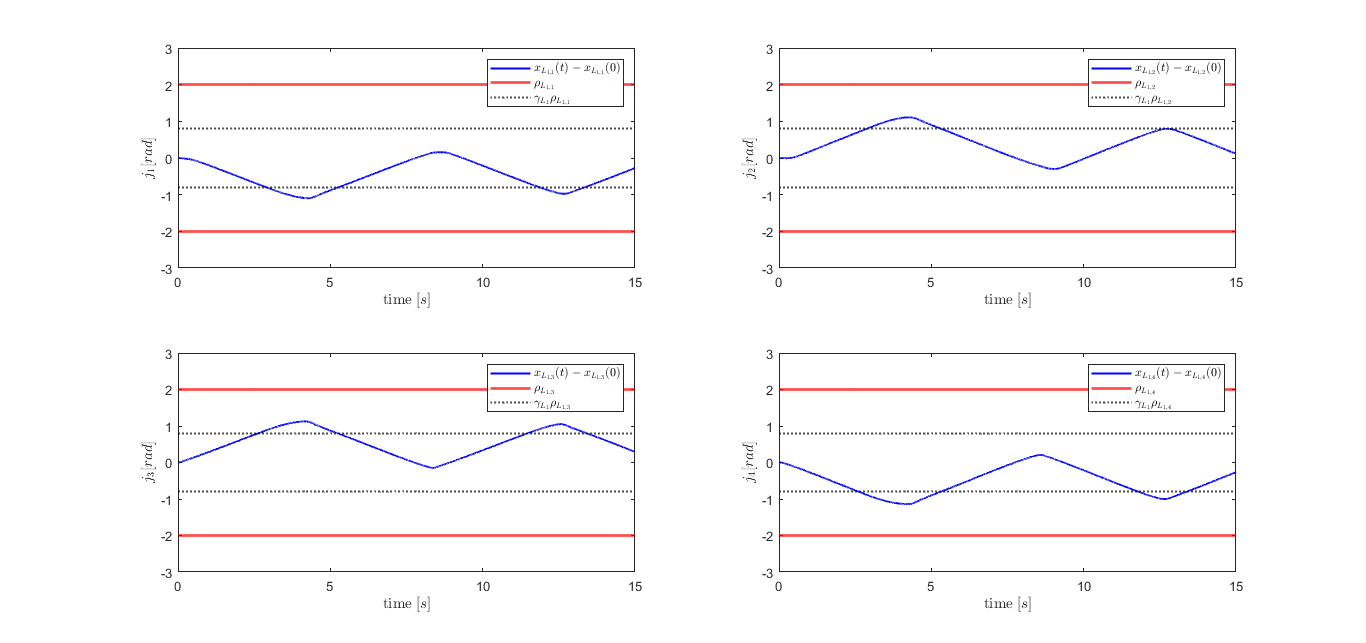
\includegraphics[width=1\linewidth]{Chapters/Chapter3/Figures/Sim2Fig7.png}
    \caption{Τα σφάλματα $x_{L_{1,i}}(t) - x_{L_{1,i}}(0)$ μαζί με τα αντίστοιχα όρια επίδοσης $\rho_{L_{1,i}}$.}
    \label{Sim2Fig7}
\end{figure}



\begin{figure}[H]
    \centering
    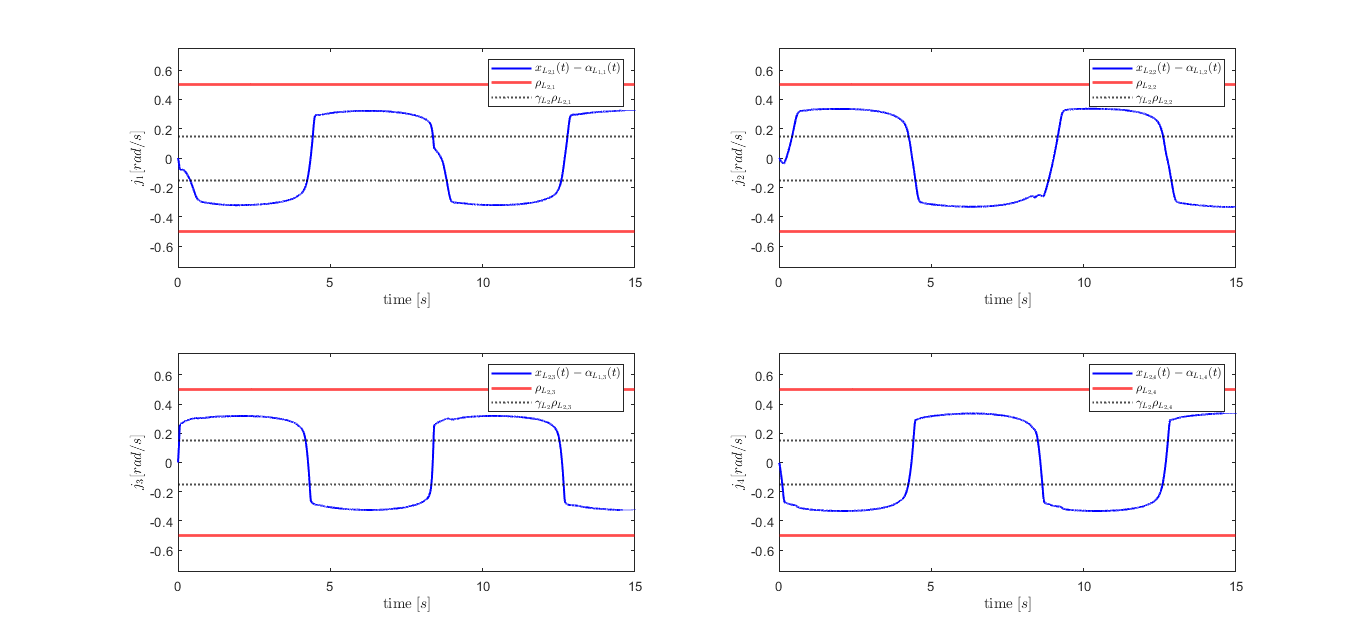
\includegraphics[width=1\linewidth]{Chapters/Chapter3/Figures/Sim2Fig8.png}
    \caption{Τα σφάλματα $x_{L_{2,i}}(t) - \alpha_{L_{1,i}}(t)$ μαζί με τα αντίστοιχα όρια επίδοσης $\rho_{L_{2,i}}$.}
    \label{Sim2Fig8}
\end{figure}

\begin{figure}[H]
    \centering
    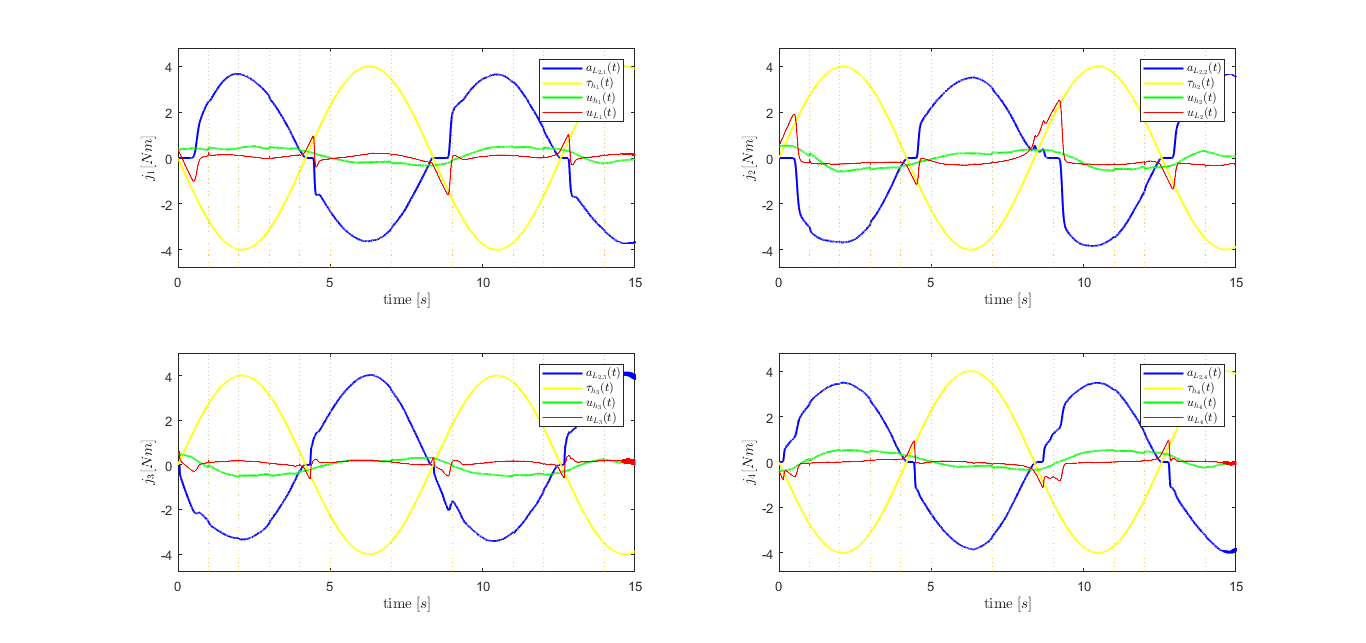
\includegraphics[width=1\linewidth]{Chapters/Chapter3/Figures/Sim2Fig9.png}
    \caption{Η είσοδος ελέγχου στον \textit{Ηγέτη} $u_{L_{i}}(t) = \alpha_{L_{2,i}}(t) + u_{H_{i}}(t)$ μαζί με τις δυνάμεις που ασκεί ο άνθρωπος πάνω του $\tau_{h_{i}}$.}
    \label{Sim2Fig9}
\end{figure}

\begin{observation} \label{figobs5}
Από τα σχήματα (\bref{Sim2Fig2}) και (\bref{Sim2Fig3}) φανερώτεται η ευρωστία του σχεδιαστικού ελέγχου παρόλι την παραβίασης της Υπόθεσης~\bref{hyp:3}. Η παρακολούθηση, αν και όχι ιδιαίτερα αυστηρή, επιτυγχάνεται, ενώ ταυτόχρονα ο Ακόλουθος διατηρείται ακέραιος, μένοντας σε απόσταση ασφαλείας από τους περιορισμούς κατάστασης εξόδου που τον οδηγουσέ ο Ηγέτης. Η επίδραση του φαινομένου αυτού είναι μηδανιμή στην συμπεριφορά του Ηγέτη (\bref{Sim2Fig7})-(\bref{Sim2Fig9}).
\end{observation}

\begin{observation} \label{figobs6}
Στο Σχήμα~\bref{Sim2Fig6}, παρατηρούνται σημαντικές αιχμές στην τιμή της εισόδου ελέγχου του Ακόλουθου κατά τις χρονικές στιγμές όπου η παράγωγος της χρονικής καθυστέρησης τείνει στο άπειρο. Ωστόσο, αυτές οι αιχμές εμφανίζονται μόνο στην Περιοχή Ασφαλείας Ακόλουθου (ΠΑΑ), όπου εφαρμόζεται η στρατηγική παρακολούθησης, και όχι στην Περιοχή Κινδύνου Ακόλουθου (ΠΚΑ). Αυτό υποδηλώνει ότι το καθεστώς ασφαλείας στην ΠΚΑ αποσβένει σημαντικές διακυμάνσεις στην είσοδο ελέγχου, αποτρέποντας τον Ακόλουθο από το να παραβεί τους περιορισμούς.
\end{observation}

\bigskip
Στο σενάριο ακραίας παραβίασης θα χρησιμοποιηθεί η καθυστέρηση με άνω φράγμα $\bar{T}_{D} = 0.3\ \text{s}$. Ύστερα από πολλαπλές δοκιμές, η ελάχιστη τιμή του φράγματος της συνάρτησης επίδοσης στην τελική κατάσταση (\bref{rhoinfty}) που παρέχει ευστάθεια στο ελεγχόμενο σύστημα ήταν από $\mathbf{0.2}$ σε $\mathbf{0.25}$ για κάθε άρθρωση.


\begin{figure}[H]
    \centering
    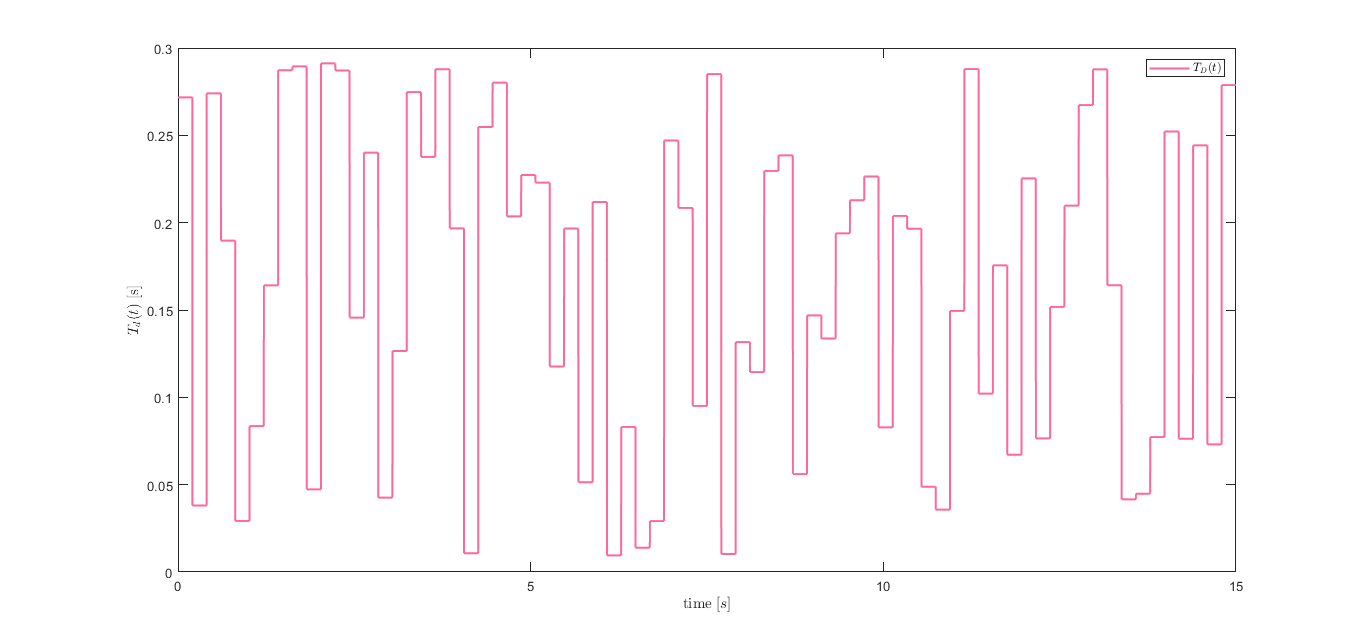
\includegraphics[width=0.9\linewidth]{Chapters/Chapter3/Figures/Sim3Fig1.png}
    \caption[Σενάριο ακραίας παραβίασης συνθηκών χρονικών καθυστερήσεων]{Σενάριο ακραίας παραβίασης συνθηκών χρονικών καθυστερήσεων}
    \label{Sim3Fig1}
\end{figure}

\begin{figure}[H]
    \centering
    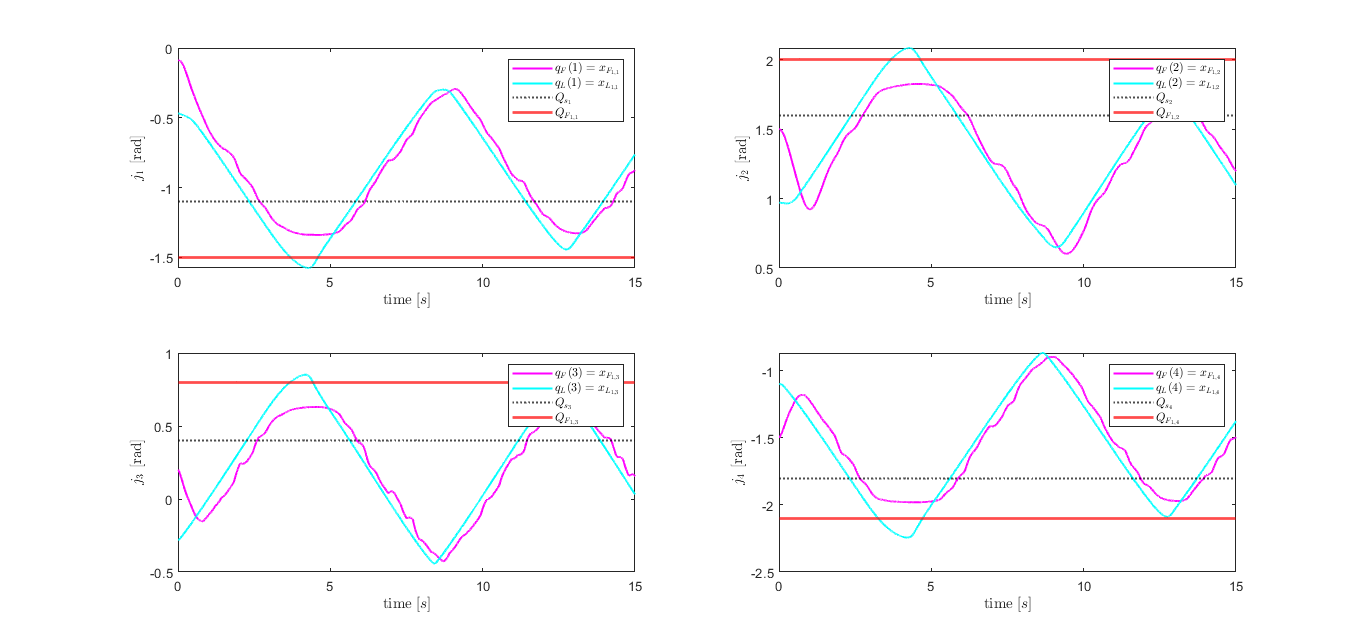
\includegraphics[width=1\linewidth]{Chapters/Chapter3/Figures/Sim3Fig2.png}
    \caption{Οι γωνίες των αρθρώσεων του \textit{Ακόλουθου} $x_{F_{1,i}}(t)$ μαζί με τις γωνίες των αρθρώσεων του \textit{Ηγέτη} $x_{L_{1,i}}(t)$.}
    \label{Sim3Fig2}
\end{figure}

\begin{figure}[H]
    \centering
    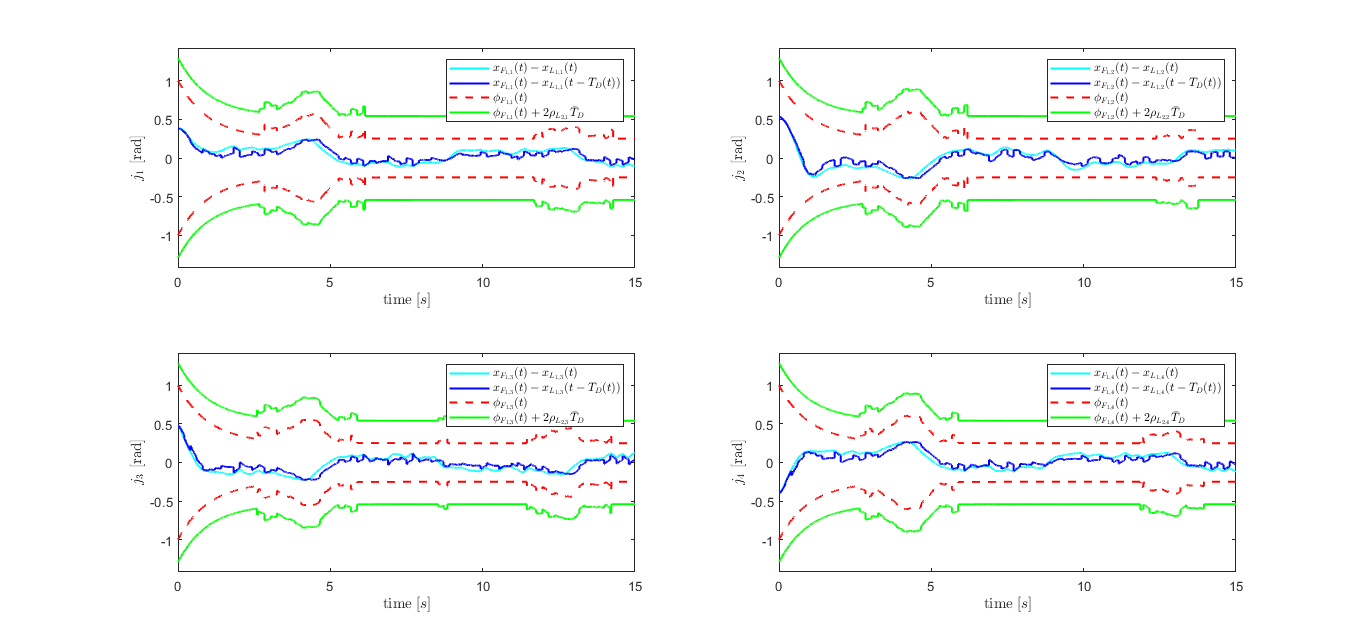
\includegraphics[width=1\linewidth]{Chapters/Chapter3/Figures/Sim3Fig3.png}
    \caption{Τα σφάλματα παρακολούθησης $x_{F_{1,i}}(t) - x_{L_{1,i}}(t - T_{D})$ και $x_{F_{1,i}}(t) - x_{L_{1,i}}(t)$ μαζί με τις αντίστοιχες συναρτήσεις επίδοσης $\phi_{F_{1,i}}(t)$.}
    \label{Sim3Fig3}
\end{figure}

\begin{figure}[H]
    \centering
    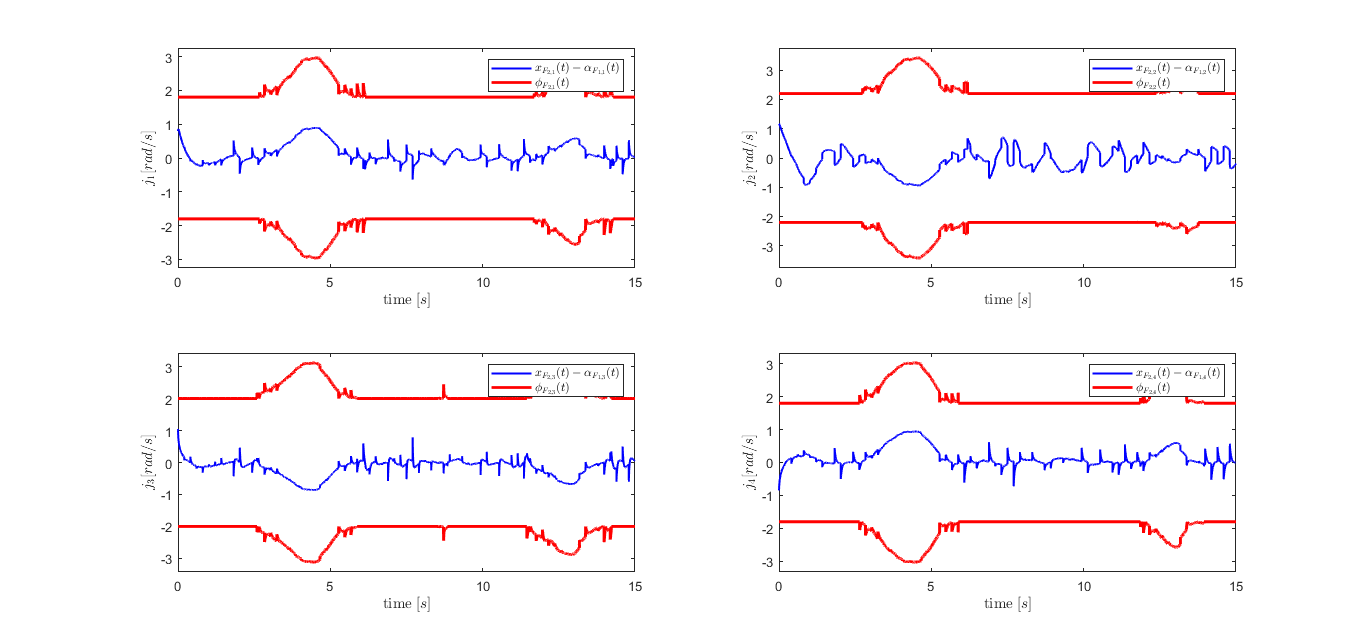
\includegraphics[width=1\linewidth]{Chapters/Chapter3/Figures/Sim3Fig4.png}
    \caption{Τα ενδιάμεσα σφάλματα $x_{F_{2,i}}(t) - \alpha_{F_{1,i}}(t)$ μαζί με τα αντίστοιχα όρια επίδοσης $\phi_{F_{2,i}}(t)$.}
    \label{Sim3Fig4}
\end{figure}

\begin{figure}[H]
    \centering
    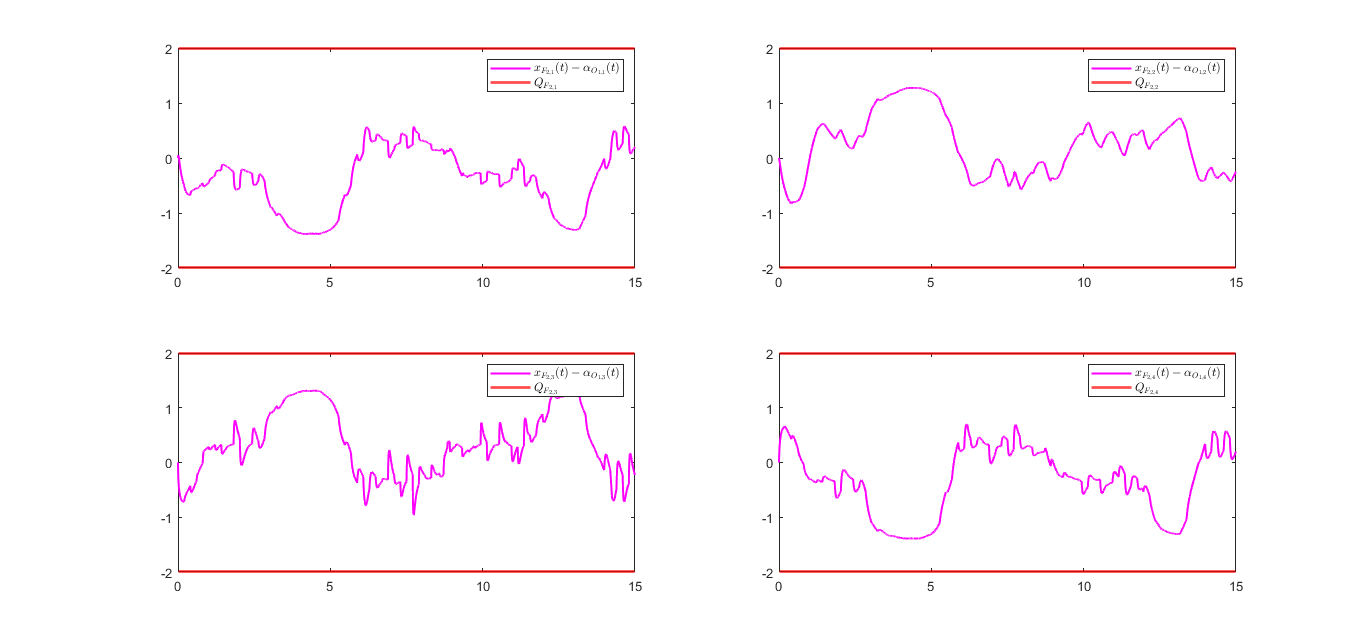
\includegraphics[width=1\linewidth]{Chapters/Chapter3/Figures/Sim3Fig5.png}
    \caption{Τα ενδιάμεσα σφάλματα $x_{F_{2,i}}(t) - \alpha_{O_{1,i}}(t)$ μαζί με τα αντίστοιχα όρια επίδοσης $Q_{F_{2,i}}$.}
    \label{Sim3Fig5}
\end{figure}



\begin{figure}[H]
    \centering
    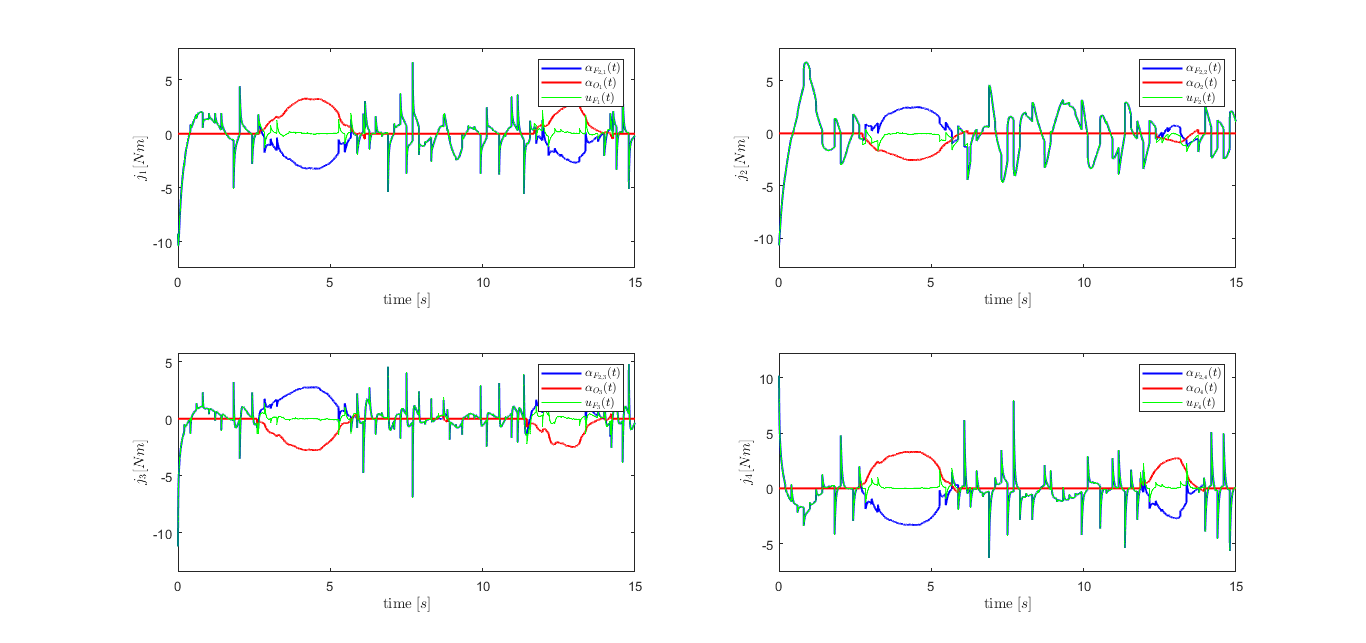
\includegraphics[width=1\linewidth]{Chapters/Chapter3/Figures/Sim3Fig6.png}
    \caption{Η είσοδος ελέγχου του \textit{Ακόλουθου} $u_{F_{i}}(t)$.}
    \label{Sim3Fig6}
\end{figure}

\begin{figure}[H]
    \centering
    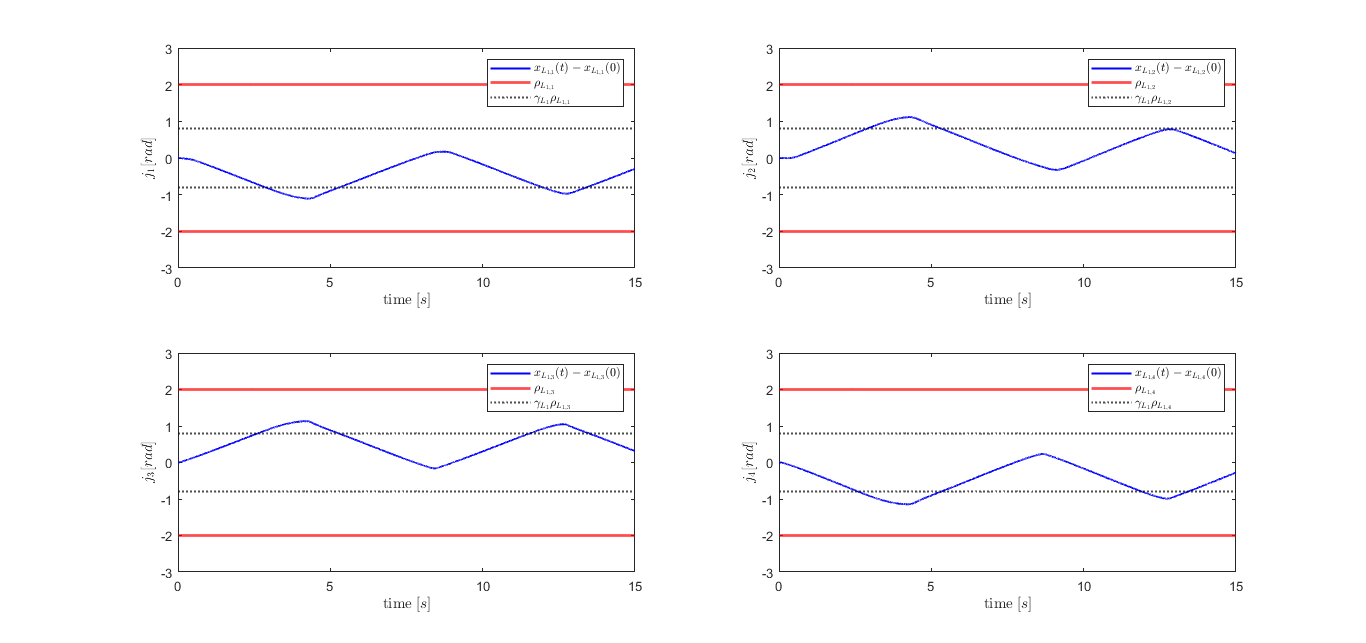
\includegraphics[width=1\linewidth]{Chapters/Chapter3/Figures/Sim3Fig7.png}
    \caption{Τα σφάλματα $x_{L_{1,i}}(t) - x_{L_{1,i}}(0)$ μαζί με τα αντίστοιχα όρια επίδοσης $\rho_{L_{1,i}}$.}
    \label{Sim3Fig7}
\end{figure}



\begin{figure}[H]
    \centering
    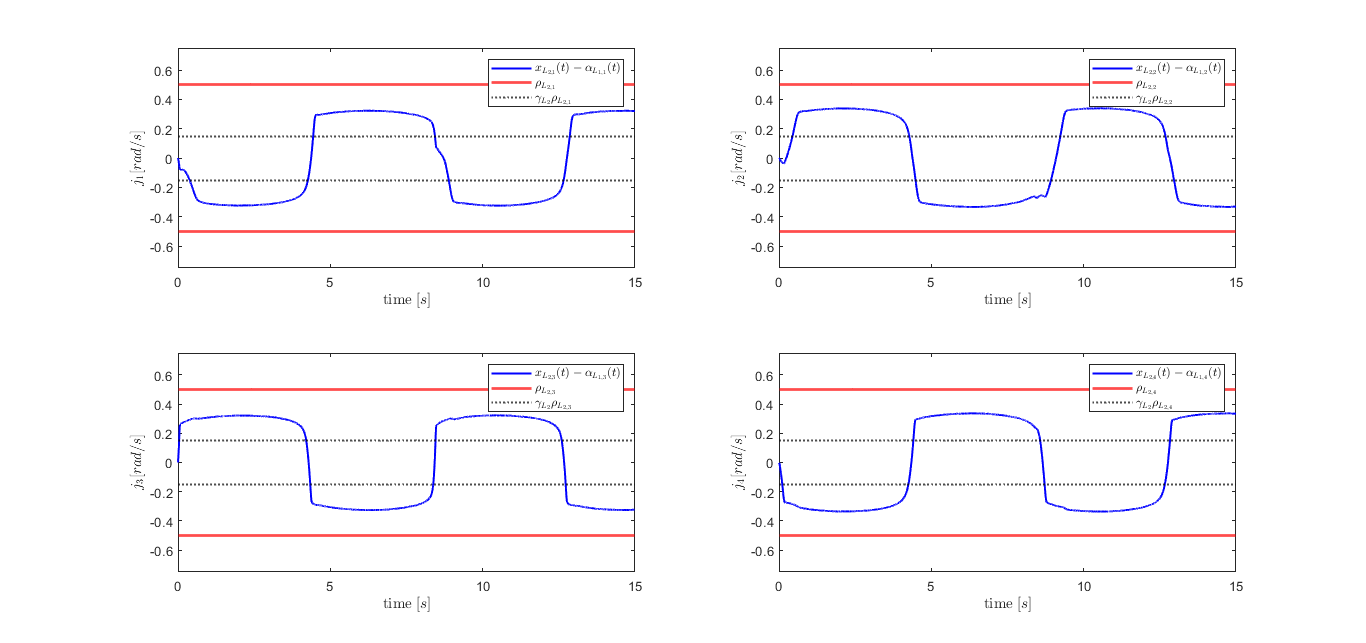
\includegraphics[width=1\linewidth]{Chapters/Chapter3/Figures/Sim3Fig8.png}
    \caption{Τα σφάλματα $x_{L_{2,i}}(t) - \alpha_{L_{1,i}}(t)$ μαζί με τα αντίστοιχα όρια επίδοσης $\rho_{L_{2,i}}$.}
    \label{Sim3Fig8}
\end{figure}

\begin{figure}[H]
    \centering
    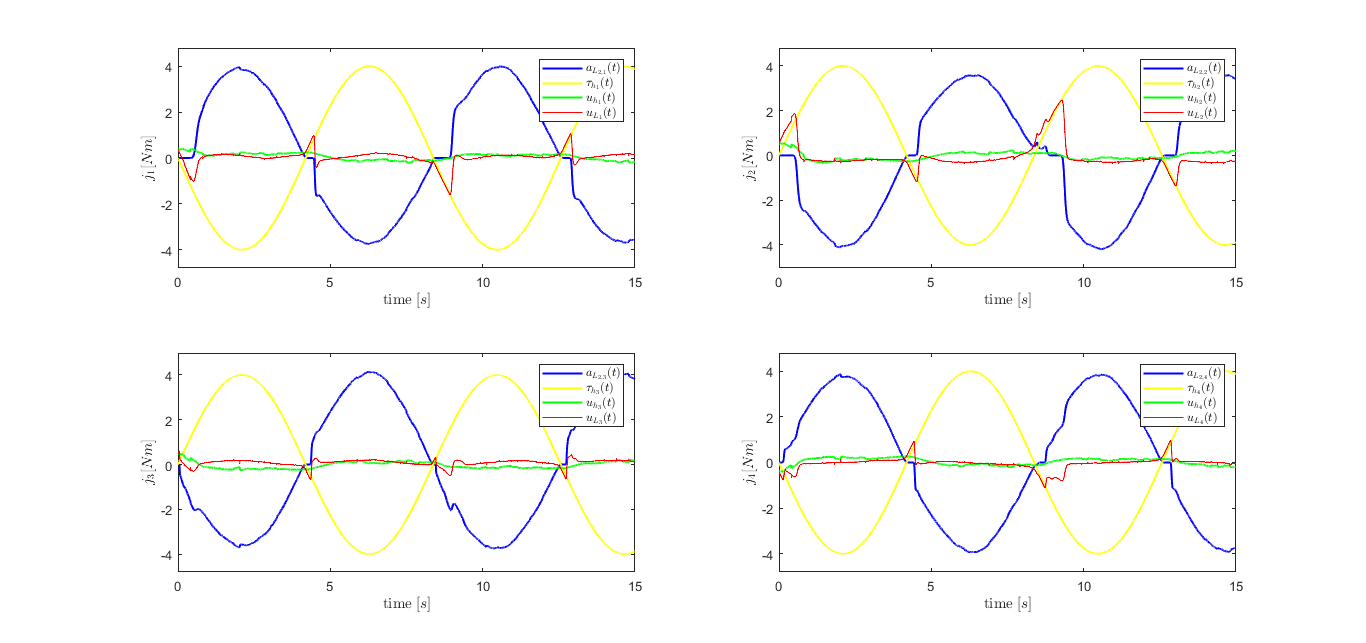
\includegraphics[width=1\linewidth]{Chapters/Chapter3/Figures/Sim3Fig9.png}
    \caption{Η είσοδος ελέγχου στον \textit{Ηγέτη} $u_{L_{i}}(t) = \alpha_{L_{2,i}}(t) + u_{H_{i}}(t)$ μαζί με τις δυνάμεις που ασκεί ο άνθρωπος πάνω του $\tau_{h_{i}}$.}
    \label{Sim3Fig9}
\end{figure}

\begin{observation} \label{figobs20} 
Από την ανάλυση όλων των σχημάτων που αφορούν τον έλεγχο του Ακόλουθου (Σχήματα~\bref{Sim3Fig2} έως~\bref{Sim3Fig6}), προκύπτει ότι, ακόμη και σε αυτή την ακραία περίπτωση, με χαμηλό άνω φράγμα στην χρονική καθυστέρηση και με σημαντική αύξηση της σχεδιαστικής παραμέτρου $\rho^{\infty}_{F_{1,i}}$, η ευρωστία και των δύο ρομποτικών συστημάτων διατηρείται, ενώ οι προδιαγεγραμμένοι στόχοι ελέγχου επιτυγχάνονται. 
\end{observation}

\begin{observation} \label{figobs21}
Στο Σχήμα~\bref{Sim3Fig6}, παρατηρούνται ακόμα πιο σημαντικές αιχμές στην τιμή της εισόδου ελέγχου του Ακόλουθου από τις αντίστοιχες στο Σενάριο~\bref{Chapter3Section3Subsection1}, οι οποίες επιφέρουν την ανάγκη της επιπλέον αύξησης του ορίου του σφάλματος εξόδου στην τελική κατάσταση. Παρόλα αυτά, και στο παρόν ακραίο σενάριο παραβίασης, εντός της Περιοχής Κινδύνου Ακόλουθου (ΠΚΑ), οι έντονες αυτές διακυμάνσεις εξουδετερώνονται σε βαθμό ικανοποιητικό που να μην παραβιάζονται οι περιορισμοί κατάστασης εξόδου.
\end{observation}

\let\cleardoublepage\clearpage